\documentclass{wileySix}
\usepackage{w-bookps}

% \usepackage{mathptmx}

\usepackage{graphicx}
\usepackage{enumitem}

\setcounter{secnumdepth}{3}

\setcounter{tocdepth}{2}

\begin{document}

\booktitle{Web Service}
\subtitle{Semua Tentang Komunikasi antar Aplikasi Berbasis Protokol internet}

\author{Rolly Maulana Awangga}

\halftitlepage
\titlepage



\offprintinfo{Web Service, pre-release}{Rolly Maulana Awangga}


\begin{copyrightpage}{2018}
Web Service / Rolly Maulana Awangga
\end{copyrightpage}


\dedication{For my family}

\contentsinbrief %optional
\tableofcontents
\listoffigures %optional
\listoftables  %optional

%%%%%%%%%
%%Content 
%%%%%%%%%

\part[Pengenalan Web Service]
{Pengenalan\\ Web Service}

%\chapter[Contoh]
%{Contoh\\ Latex}
%\prologue{The sheer volumne of answers can often stifle insight...The purpose
of computing\index{computing!the purpose} is insight, not numbers.}
{Hamming}

\section{Definisi Web Service}
Web service adalah suatu sistem perangkat lunak yang dirancang untuk mendukung interoperabilitas dan interaksi antar sistem pada suatu jaringan. Web service digunakan sebagai suatu fasilitas yang disediakan oleh suatu web site untuk menyediakan layanan (dalam bentuk informasi) kepada sistem lain, sehingga sistem lain dapat berinteraksi dengan sistem tersebut melalui layanan-layanan (service) yang disediakan oleh suatu sistem yang menyediakan web service. Web service menyimpan data informasi dalam format XML, sehingga data ini dapat diakses oleh sistem lain walaupun berbeda platform, sistem operasi, maupun bahasa compiler.

Web service bertujuan untuk meningkatkan kolaborasi antar pemrogram dan perusahaan, yang memungkinkan sebuah fungsi di dalam Web Service dapat dipinjam oleh aplikasi lain tanpa perlu mengetahui detil pemrograman yang terdapat di dalamnya.

Beberapa alasan mengapa digunakannya web service  adalah sebagai berikut:

-Web service dapat digunakan untuk mentransformasikan satu atau beberapa bisnis logic atau class dan objek yang terpisah dalam satu ruang lingkup yang menjadi satu, sehingga tingkat keamanan dapat ditangani dengan baik. 

-Web service memiliki kemudahan dalam proses deployment-nya, karena tidak memerlukan registrasi khusus ke dalam suatu sistem operasi. Web service cukup di-upload ke web server dan siap diakses oleh pihak-pihak yang telah diberikan otorisasi.

-Web service berjalan di port  80 yang merupakan protokol standar HTTP, dengan demikian web service tidak memerlukan konfigurasi khusus di sisi firewall.\cite{awangga2017colenak}.

\section{Sejarah Web Service}
Penemu website adalah Sir Timothy John ¨Tim¨ Berners-Lee, sedangkan website yang tersambung dengan jaringan, pertamakali muncul pada tahun 1991. Maksud dari Tim ketika membuat website adalah untuk mempermudah tukar menukar dan memperbarui informasi kepada sesama peneliti di tempat dia bekerja. Pada tanggal 30 April 1993, CERN (tempat dimana Tim bekerja) menginformasikan bahwa WWW dapat digunakan secara gratis oleh semua orang. Sebuah website bisa berupa hasil kerja dari individu, atau menunjukkan kepemilikan dari sebuah organisasi, perusahaan, dan biasanya website itu menujukkan beberapa topik khusus, atau kepentingan tertentu. Sebuah website bisa berisi hyperlink yang menghubungkan ke website lain, jadi, kadang sulit membedakan antara website yang dibuat oleh individu perseorangan dengan website yang dibuat oleh organisasi bisnis bisa saja tidak kentara.

Website yang ditulis di konversi menjadi HTML oleh komputer dan diakses melalui web browser, yang dikenal juga dengan HTTP Client. Halaman web dapat dilihat atau diakses melalui jaringan komputer dan internet, perangkatnya bisa saja berupa komputer pribadi, laptop, PDA ataupun telepon selular.

Sebuah website dibuat didalam sebuah sistem komputer yang dikenal dengan server web, juga disebut HTTP Server, dan pengertian ini juga bisa menunjuk pada software yang dipakai untuk menjalankan sistem ini, yang kemudian menerima lalu mengirimkan halaman-halaman yang diperlukan untuk merespon permintaan dari pengguna. Apache adalah piranti lunak yang biasa digunakan dalam sebuah webserver, kemudian setelah itu adalah Microsoft Internet Information Services.



\subsection{Sir Timothy John ¨Tim¨ Berners-Lee}
Pada tanggal 30 April 1993, CERN (tempat dimana Tim bekerja) menginformasikan bahwa WWW dapat digunakan secara gratis oleh semua orang.

\begin{figure}[ht]

\centerline{\includegraphics[width=1\textwidth]{figures/petaduniaalid.JPG}}
\caption{Gambaran pengantar peta dunia karya al-Idrisi tahun 1154.}
\end{figure}

\begin{figure}[ht]
	\centerline{\includegraphics[width=1\textwidth]{figures/TabulaRogeriana.jpg}}
\vskip2pt
\caption{Tabula Rogeriana digambar oleh Al-Idrisi pada tahun 1154 untuk Raja Normandia Roger II dari Sisilia, setelah delapan menetap di istananya, di mana dia bekerja untuk penjelasan dan ilustrasi peta.}
\end{figure}




%\chapter[Internet]
%{Definisi\\ Internet}
%\input{section/1internet.tex}

%\chapter[Web]
%{Definisi\\ Web}
%\documentclass[12pt, a4paper]{article}
\linespread{1.5}


\title{World Wide Web}
\maketitle

%\begin{itemize}
%\item Imron Sumadireja (1164076)
%\item Jesron Marudut (1164077)
%\item Lusia Violita Aprilian (1164080)
%\item Mhd. Zulfikar Akram Nst. (1164081)
%\end{itemize}

\section{Pengertian Website}
World wide web (www atau web) merupakan halaman situs informasi yang dapat diakses secara cepat atau sarana
antar muka informasi di internet. Web dapat menggabungkan teks, grafik, dan multimedia. Web memudahkan
penggunanya untuk mengakses informasi melalui konsep hypertext sehingga memungkinkan  suatu text untuk
menjadi acuan membuka dokumen laindo. Informasi dapat mudah disebar dan diakses.

\subsection{Sejarah Website}
Sementara itu World wide web (www) dikembangkan pertama kali oleh Tim Berners-Lee pada tahun 1989. Pada
awalnya, Tim mengusulkan WWW sebagai suatu cara berbagai dokumen diantara para peneliti. Dokumen online dapat
diakses melalui alamat unik yang disebut Universal Resource Locator atau URL. Selain itu WWW tidak hanya
dikembangkan untuk keperluan para peneliti, namun juga dikembangkan untuk kalangan pendidikan, bisnis dan
perorangan. Berdasarkan penjelasan singkat diatas dapat disimpulkan bahwa antara web dan internet memiliki
hubungan yang sangat erat walaupun keduangnay tidak bisa dikatakan sama. Web merupakan bagian dari layanan
yang dapat berjala di atas teknologi internet.

\subsection{Jenis-jenis website}
Website dikelompokan dalam beberapa jenis-jenis Website agar dapat memudahkan dalam menentukan jenis website
yang akan ditentukan. Dan berikut jenis-jenis website yang dikelompokan atas beberapa dasar:
\begin{enumerate}
\item Jenis Website berdasarkan sifat;
\begin{itemize}
\item Website Statis, merupakan web yang kontenya hampir jarang diubah
\item Website Dinamis, Web yang konten atau isinya dapat berubah-ubah setiap saat
\end{itemize}
\item Jenis Website yang dikelompokkan berdasarkan Bahasa Pemrogramannya;
\begin{itemize}
\item Server side, Website yang memakai bahasa pemrograman yang tergantung dengan servernya
\item Client side, adalah web yang tidak perluu server untuk menjalankannya. Cukup diakses dengan browser.
\end{itemize}
\item Jenis-jenis Web menurut tujuannya;
\begin{itemize}
\item Web personal, biasanya web ini merupakan web yang berisi informasi seorang
\item Corporate Web, website yang dimiliki sebuah institusi atau perusahaan.
\item Web Portal, Web ini berisi banyak layanan, seperti berita, email dan jasa
\item Web Forum, sebuah web yang dibuat sebagai sarana diskusi.
\end{itemize}
\end{enumerate}
	
\subsection{Keuntungan Web}
Keuntungan penggunaan web diantaranya yaitu :
\begin{itemize}
\item Informasi dapat diberikan segera(tepat waktu) dan diperbarui secara berkala.
\item Presentasi fleksible dan visibilitas dapat menyediakan ragam isyarat untuk diseminasi informasi.
\item Informasi dapat diorganisir melalui tautan dan menu, berbagai tingkatan informasi dapat disediakan format file yang berbeda dapat digunakan untukj informasi yang dapat diunduh. Integrasi informasi dapat dilakukann melalui tautan dan seksi lain, halaman lain, atau web lain.
\item Tauta  dan menu dapat menyediakan informasi bagi pemangku kepentingan yang berbeda, informasi dapat pula diberikan melalui daftar email kepada pemangku kepentingan.
\item Setiap orang yang dapat mengakses web dapat memperoleh informasi karena keterjangkauan global dan potensi komunikasi masl dari web.
\end{itemize}
	   
\section{tentang web scraping}
Web scraping atau scraping web (dapat disebut juga panen web atau web ekstraksi data) merupakan sebuah
perangkat lunak komputer teknik penggalian informasi dari situs web seperti mengambil mengambil data
berbentuk teks yang umumnya bertipe HTML atau XHTML. contohnya seperti Internet Explorer (IE) dan Mozilla Web
Browser. web scraping berkaitan erat dengan pengindekan web.

\subsection{manfaat dari web scraping}
Web scraping sering dikenal dengan screen scraping. Web scraping tidak dapat dimasukkan kedalam bidang data
mining karena dalam data mining menyiratkan upaya untuk memahami pola semantik dari sejumlah data besar yang
telah diperoleh. Aplikasi Web scraping hanya fokus pada cara memperoleh data melalui pengambilan dan ekstrasi
dengan ukuran data yang bervariasi. Manfaat dari web scraping adalah agar informasi yang diambil lebih
terfokus sehingga dapat memudahkan dalam melakukan pencarian sesuatu, adapun cara untuk mengembangkan teknik
web scraping yaitu dengan cara sebagai berikut:
\begin{enumerate}
\item Pengembang/pembuat program mempelajari dokumen HTML dari website yang akan diambil informasinya untuk
di tag HTML tujuannya yakni untuk mengapit informasi yang akan diambil (Create Scraping Template)
\item Pengembang/pembuat program mempelajari teknik navigasi pada website yang akan diambil informasinya
untuk ditiru pada aplikasi web scraping yang akan dibuat (Explore Site Navigation)
\item Selanjutnya aplikasi web scraping akan mengotomisasi informasi yang didapatkan dari website yang telah
ditentukan (Automate Navigation and Extraction), informasi yang didapat tersebut akan disimpan dalam 
tabel basis data (Extracted Data and Package History).
\end{enumerate}

\subsection{Perbandingan Metode Web Scraping}
Berikut perbandingan antara metode Web Scraping menggunakan CSS Selector dan Xpath Selector
\begin{enumerate}
\item Penggunaan metode XPATH Selector untuk web scraping menghasilkan artikel yang lebih lengkap
dibandingkan dengan menggunakan metode CSS Selector, Ditunjukkan dengan jumlah item dan ukuran file
yang didapatkan lebih besar. Namun juga menyisakan proses lain untuk menghilangkan kode HTML yang tidak
diinginkan dari artikel yang dihasilkan menggunakan metode XPATH Selector.
\item Dalam penggunaan memori baik metode XPATH Selector dan CSS Selector tidak memiliki perbedaan yang
signifikan(cenderung sama). Disebabkan karena engine scrapy yang baik dalam penggunaan resource-nya. 
\item Metode XPATH Selector memiliki waktu proses yang lebih cepat daripada menggunakan metode CSS Selector.
\item Pada metode XPATH, selector cukup mengikuti node pada halaman web, sehingga waktu yang dibutuhkan
relatif lebih singkat.
\end{enumerate}

\section{Tentang Web Hosting}
Web hosting merupakan jasa penyewaaan tempat penyimpanan data di internet atau biasa disebut dengan cloud
yang diperlukan oleh sebuah website. Web hosting ialah salah satu syarat agar website bisa diakses secara 
online dan dapat diakses dari seluruh dunia. Ukuran yang digunakan dalam suatu web hosting adalah kapasitas
dan bandwidth. Kapasistas merupakan ukuran besarnya kemampuan sebuah web hosting untuk menyimpan data-data di internet.

Bandwidth merupakan ukuran maksimal dari jumlah volume data yang diperbolehkan untuk diakses dari web hosting
setiap bulannya. Sebagai contoh, sebuah halaman website yang mempunyai ukuran 2 MB dan bandwidth web hosting
2000 MB, maka setiap bulannya website tersebut dapat diakses sebanyak 2000 kali.

\subsection{Tentang Domain}
Domain merupakan sebuah alamat di dunia internet atau sebuah identitas dari sebuah website. Domain digunakan untuk mempermudah dalam mengakses situs yang ada di internet. Domain terbagi menjadi 2 jenis domain yang dibagi berdasarkan pemisahaan titiknya, yaitu; Top Level Domain (TLD) dan Second Level Domain (SLD). Top Level Domain merupakan bagian terakhir dalam sebuah domain website. Contohnya "facebook.com" dan disitu yang jadi domainnya adalah ".com". Selanjutnya Second Level Domain atau SLD merupakan bagian dari domain yang terdapat sebelum Top Level Domain. Contohnya "Facebook.com" yang menjadi SLDnya adalah Facebook. Jadi SLD adalah unsur domain yang didaftarkan terdahulu pada jasa Web Hosting. Dan ada juga yang disebut Country Code Second Level Domain (ccSLD). Berguna sebagai penunjuk organisasi apa yang mendaftar pada suatu domain. Setiap negara juga mempunyai ccSLD yang berbeda-beda tiap negaranya.

\subsection{Tentang Hubungan Domain dan Web Hosting}
Hubungan Domain dan Web Hosting merupakan satu kesatuan yang saling membutuhkan. Pada sebuah Website, domain dan web hosting saling ketergantungan. Apabila yang tersedia hanya web hosting, maka website tidak akan dapat diakses. Begitu juga dengan domain, apabila yang tersedia hanya domain, maka tidak akan ada website yang akan ditampilkan, karena halaman website tersimpan didalam web hosting.

\subsection{Macam-macam Web Hosting}
Saat ini banyak jasa penyedia hosting dengan harga relatif murah bahkan gratis. Berikut adalah macam-macam web hosting :
\begin{enumerate}
\item Free Hosting / Web Hosting Gratis
Dengan free hosting, kita dengan mudah mencari layanan web hosting dan domain gratis di internet dengan menggunakan fasilitas search engine seperti google atau yang lainnya. Biasanya penyedia web hosting tidak mengenakan biaya. Namun, memiliki banyak keterbatasan beberapa fitur.
\item Web Hosting Berbagi atau Shared Hosting
Jenis hosting ini paling sering digunakan karena bukan hanya murah, namun juga memiliki layanan yang  dapat mencukupi segala kebutuhan. Biasanya, untuk menggunakan layanan web hosting ini anda hanya perlu untuk mengeluarkan biaya sebesar 100 hingga 200 ribu untuk mendapatkan ruang sebesar 2 GB – 7,5 GB dengan bandwith unlimited.
\item VPS Web Hosting
VPS merupakan singkatan dari Virtual Private Server. Jadi disini anda dapat seperti memiliki server sendiri untuk situs anda. dengan server ini, anda akan memiliki control yang lebih dalam seperti Dedicated Server.
\item Dedicated Web Hosting
Dedicated Web Hosting merupakan sebuah layanan hosting dengan server yang memiliki kemampuan untuk melakukan handle terhadap traffic dengan jumlah sangat banyak. Serta memiliki banyak fitur premium di dalamnya. Selain itu,juga memiliki control penuh terhadap server walaupun  hanya menyewanya.
\item Managed Web Hosting
Managed Hosting / Web Hosting Terkelola ini adalah web hosting yang dikhususkan untuk situs dengan. Platform yang sama. Managed web hosting biasanya lebih aman dan kinerjanya lebih optimal. Selain itu, memudahkan untuk melakukan beragam pengaturan, mulai dari installasi, sampai setting macam-macamnya.
  \end{enumerate}

\subsection{Cara Mendapatkan Web Hosting dan Domain}
Web hosting dan domain lebih sering ditemukan oleh perusahaan-perusahaan penyedia web hosting atau domain. Untuk menemukannya, cukup cari di google. Maka akan banyak perusahaan yang menyediakan jasa web hosting. Kinerja web hosting berbeda-beda dari setiap perusahaan Web hosting. Karna apabila web hosting yang dibuat oleh jasa tersebut buruk maka website tersebut akan mudah bermasalah. Oleh karena itu dalam pembelian jasa domain atau web hosting perlu diperhatikan hal-hal seperti profil dari penjual web hosting, fitur untuk website dan harga dari web hosting tersebut. Dalam memilih penyedia web hosting, pastikan penyedia mempunyai reputasi yang bagus dan terpercaya. Dan sebaiknya memilih perusahaan web hosting yang sudah dalam bentuk perusahaan CV atau PT agar pertanggung jawabannya jelas ketika terjadi gangguan web hosting.
	
\section{Apa itu cPanel?}
Apa itu cPanel?
cPanel adalah perangkat lunak control panel online untuk melakukan pengaturan website dalam sebuah web histing. cPanel adalah tool utama untuk pengguna web hosting. 
Beberapa fungsi utama cPanel antara lain yaitu upload data website, pengaturan data website, instalasi content management system, dan lain-lain. Melelui cPanel juga kita bisa mengatur data-data website. Kita bisa menambah, menghapus, atau memodifikasi data website.

\subsection{Backup date dengan cPanel}
Kemudahan yang diberikan cPanel sebagai control panel yakni untuk mempermudah proses hosting di suatu situs web menggunakan 3 tingkatan struktur untuk memberikan fungsi administrator, agen, dan yang memiliki situs web tersebut untuk mengatur berbagai macam aspek dari situs web dan administrasi server melalui sebuah web standar. Dalam menu cPanel untuk backup disediakan 3 pilihan layanan backup yang ada yakni:
\begin{enumerate}
\item System Backup, merupakan menu backup yang dapat digunakan untuk mendownload backup otomatis yang telah dibuat oleh administrator server
\item Full Backup, akan melakukan backup file untuk mengembalikan file yang corrupt, terhapus atau pindah pada server yang lain.
\item Backup Home Directory, berfungsi untuk memberikan hak akses untuk mengambil file yang berada pada directory home.
\end{enumerate}


\chapter[Backend]
{Definisi\\ Backend}


\section{Backend}

\begin{figure}[ht]
\centerline{\includegraphics[width=1\textwidth]{figures/1backend.jpg}}
\caption{Backend}
\label{1backend}
\end{figure}

	Pada gambar \ref{1backend} berikut ini dijelaskan mengenai Back-end atau server-side yang merupakan bagaimana sebuah website berkerja, meng-update
dan berubah. back-end adalah sesuatu system yang dimana User tidak akan dapat melihatnya di dalam browser,
seperti Database dan Server. biasanya orang - orang yang bekerja di bagian back-end di panggil atau disebut sebagai
Programmers atau Developer. Back-end developers adalah orang yang paling khawatir tentang hal - hal yang menyangkut keamanan,
struktur sistem dan manajemen konten. sebenarnya para back-end develper juga mengetahui tentang front-end seperti HTML dan CSS.
namun itu bukanlah bidang mereka bekerja. 

\subsection{Backend System}
	Pada system dan metode  yang membuat informasi dapat digunakan secara oromatis untuk mengakses 
pada fungsionalitas system computer backend yang digunakan ke server aplikasi. 
Metode ini juga dapat beroperasi untuk menghubungkan ke system computer backend dan memperoleh 
fungsionalitas untuk menentukan informasi  pada system backend. Dan pada informasi yang diperoleh 
dan dapat dianalisis secara terprogram,dan informasi yang sangat baru dapat dianalisis yang dimana 
informasi dibuat secara terprogram dapat digunakan untuk mengakses fungsionalitas system backend.
Back-end biasanya mengacu pada program dan skrip yang bekerja di dalam server, untuk membuat sebuah 
halaman web yang dinamis dan interatif. Back-end memiliki tugas-tugas yaitu seperti :

\begin{enumerate}
\item Desain Informasi pada web
\item Pemrosesan form
\item Pemrograman dalam database
\item Aplikasi Berbasis Web
\end{enumerate}
Dari tugas - tugas tersebut Back-end memiliki tiga bagian diantaranya yaitu server,aplikasi, dan database
\cite{shapiro2005system}.

\section{Bahasa Pemrograman yang digunakan di Backend}
Pada gambar \ref{2labelgambar} berikut ini dijelaskan bahwa pada Backend terdapat beberapa bahasa programing yang digunakan,
termasuk C, Python, dan lainnya. pada materi di bawah ini terdapat beberapa penjelasan tentang bahasa pemrogramannya.

\begin{figure}[ht]
\centerline{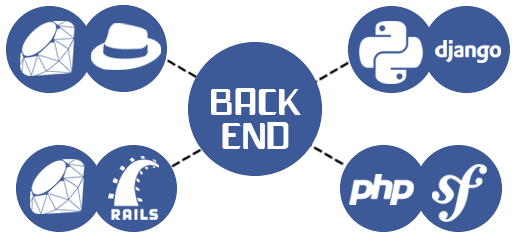
\includegraphics[width=1\textwidth]{figures/1bahasapemrogramanbackend.png}}
\caption{Bahasa Pemrograman yang dipakai di Backend}
\label{2labelgambar}
\end{figure}

\subsection{C}
	Bahasa Pemrograman Backend yang biasa digunakan developer ialah C, C++, dan Java .
Bahasa C adalah suatu perkembangan dari bahasa B yang di kembangkan oleh Ken Thompson pada tahun 1980.
Bahasa C rilis pertama kali ditulis oleh Brian W. Bahasa C, awalnya digunakan oleh sistem operasi UNIX.
Bahasa C adalah bahasa pemrograman tingkat standar, bahasa C memiliki kegunaan yang sering di gunakan
diantaranya untuk membuat perangkat lunak.

\subsection {C++}
	Pengertian C++ adalah `multi-paradigm' artinya anda dapat menulis suatu kode, caranya procedural 
tapi juga bisa menggunakan fungsional,berorientasi objek, dan campuran paradigm suatu pemrograman.  
Bahasa pemrograman C++ ini bisa lebih sulit untuk dipelajari; kita dapat mengembangkan dengan 
menggunakan satu atau lebih dari model ini,  atau kita dapat menggabungkan dengan Bahasa pemrograman lainnya.

\subsection {C\#}
	Sedangkan C\# merupakan sebuah bahasa programming yang simple, modern, OOP dan aman untuk 
penggabungannya dengan beberapa bahasa programming lain
\cite{hejlsberg2003c}.

\subsection {PHP}
 	adalah salah satu server side untuk dirancang khusus untuk aplikasi web dan PHP disisipkan diantara bahasa HTML sebab bahasa server side, maka dieksekusi diserver. sehingga yang kirimkan ke browser adalah hasil jadi dalam bentuk HTML. PHP termasuk Open Source Product dapat diubah disource code dan mendistribusikan secara bebas.

\subsection{Python}
	Python merupakan  bahasa pemrograman yang serba guna atau bersifat open source. 
Python lebih menekankan pada pembacaan  kode agar lebih mudah untuk memahami sintaks. 
Hal tersebut membuat bahasa pemrograman python lebih mudah dipelajari baik pemula maupun untuk yang 
sudah menguasai bahasa pemrograman ini dan dilengkapi dengan fungsionalitas standar besar serta 
komprehensif. Pyhton telah digunakan untuk mengembangkan berbagai macam perangakat lunak, seperti 
internet scipting, system programming, user interfaces, prudect customization,numberic programming. 
Pada saat ini bahasa pemrograman pyhton menduduki posisi 4 atau 5 paling sering digunakan diseluruh dunia.

\subsection{Perl}
	Proxy server ialah suatu komputer atau beberapa komputer yang diletakkan sebagai pelayanan kepada pelanggan yang ingin mengajukan layanan data baik dari pusat komputer(server).
Proxy server sering disebut sebagai media cache terhadap suatu konten website. Di ruang lingkup pendidikan pada laboratorium komputer jaringan di Institusi Sains \& Teknologi ditemukan jaringan yang belum ada penanganan masalah internet yang diakses berkali-kali sehingga bandwidth pada internet tidak efektif, penelitian ini bertujuan  untuk melakukan suatu penyimpanan konten yang diakses ke dalam proxy server kemudian melakukan filter konten menggunakan pemrograman PERL.
Ini dilakukan melalui proxy server, yaitu melalui fungsi pada cachig dan filter pada proxy server dengan menggunakan pemrograman PERL dan regex pada PERL
\cite{pamungkas2017implementasi}.

\subsection{ASP .NET}
	ASP.NET merupakan produk dari teknologi Microsoft untuk pengembangan aplikasi berbasis web dinamis. 
Bahasa pemrograman ini mempermudah pada pemula maupun yang sudah menguasai bahasa pemrograman ini , dikarenakan memberikan solusi pada pengembang untuk mendesign aplikasi web dengan cepat, mudah dan efisien. 
ASP diproses melalui web server dan menghasilkan HTML untuk dikirimkan pada web browser.


\subsection{Java}
	Dalam backend juga menggunaka javascript yaitu suatu format teks untuk mengserialisasi data yang terstruktur yang berasal dari objek literal JavaScripts.Pada JavaScript dapat mewakili dari empat tipe yaitu string, angka, boolean, dan nul, dan ada juga dua tipe terstruktur yaitu objek dan array. Objek kumpulan yang tanpa batas dari nol ata lebih dari nama atau nilai pasangannya, yang dimana nama ialah string sedangkan nilai ialah angka, boolean, objek, dan null. Array yaitu urutan dari nol atau melebihi banyak nilai.

\subsection{Ruby}
	Ruby merupakan bahasa pemrograman yang stabil, dengan menggabungkan bahasa pemrograman favoritnya seperti Perl, smalltalk, Eiffel, dan Lisp.
Membentuk suatu bahasa pemrograman baru yang menyeimbangkan pemrograman fungsional dengan imperatif.
Bahasa pemrograman Ruby mempunyai sistem yang dengan otomatis akan langsung terhapus semua data-data yang tidak terpakai dan tidak digunakan lagi pada memori. 
Platform sistem operasi yang mendukung bahasa pemrograman Ruby yaitu sistem operasi Linux, Unix, Amiga, Symbian, Mac dan Windows.

\section{Database Backend}
	Pada sistem basis data yaitu telah lama dilanda masalah kinerja pada penigkatan dalam penggunaan mainframe atau di dalam aplikasi basis data. Dan solusi untuk masalah ini yaitu dengar membongkar sistem basis data dari komputer mainframe ke komputer backend. Pada komputer itu memiliki penyimpanan disk sendiri, digunakan juga untuk melakukan semuoa operasi data base, dan saling berinteraksi dengan mainframe
\cite{yousefi2008database}.


\section{Arsitektur Three-Tier}
	Didalam masalah arsitektur two-tier telah diupdate ke tingkat tertentu dengan memperluas dari dua tingkat menjadi tiga tingkat.
Arshitektur three-tier akan mengisolisasi pemrosesan data dari lokasi pusat yang dapat dengan mudah diubah tanpa melibatkan dan mepengaruhi klien. Di dalam arsitektur three-tier ini, logika presentasi berada pada tingkat pertama (klien), logika bisnis berada pada 
tingkat menengah, dan yang lainnya seperti database berada di tingkatan ketiga yaitu back-end. Di tingkat menengah dalam
arsitektur three -tier (server aplikasi) akan menangani pemrosesan data dan akan menjadi antarmuka antara front - end (klien) dan
tingkat back-end (database)
\cite{demurjian1986multi}.


\section{Web Service}
	Web Service merupakan penyatuan dari 2 aspek yaitu Web dan Service, yang mana penjelasan Web dan Service akan dijelaskan di bawah ini :

\subsection{Web}
	pertama - tama disini akan dijelaskan tentang Web, Web merupakan website yang berarti 
jaringan yang dapat mengakses situs secara global.

\subsection{Service}
	Service merupakan layanan, yang dimana digunakan untuk melayani dan melakukan pelayanan.
sehingga dari kedua perihal diatas dapat disimpulkan bahwasanya web service adalah sebuah jaringan global yang memiliki pelayanan atau keamanan,
didalam web service user diberikan layanan berupa keamanan dalam berselancar di Internet. 
macam - macam model dari web service adalah sebagai berikut ini :

\begin{enumerate}
\item SOAP (Simple Object Access Protocol)
\item WDSL (Web Service Description Language)
\item RDF (Resource Description Framework)
\item RSS (Really Simple Syndication)
\end {enumerate}
\cite{curbera2001web}.


\section{Backend Developer}
	Orang yang bekerja di bagian back-end atau bisa kita sebut seorang back-end developer adalah seorang programmer yang hanya
memusatkan atau berfokus pada bagian keamanan, desain sistem, dan management data pada sistem. Seorang back-end developer
sangat dibutuhkan dalam melakukan pengembangan sistem atau sebuah aplikasi yang dinamis atau aplikasi yang memiliki data selalu
berubah - ubah, contohnya website yang dinamis seperti facebook dan google.

\section{Backend as a Service}
	Baas adalah sebuah provider untuk web dan mobile app developer untuk dapat mengkoneksikan 
aplikasi mereka ke dalam system penyimpanan cloud backend sekaligus masih tetap melakukan proses yang lain seperti user management, 
mendapatkan notifikasi, bermain social media, dan fitur – fitur lainnya yang terdapat di dalam aplikasi mobile mereka saat ini.

\subsection{Kelebihan yang dimiliki BaaS}
	Tujuan dari BaaS adalah untuk membuat hidup developer menjadi 
lebih mudah. BaaS ada karena kurangnya keahlian dari seorang 
mobile developer dan tingginya tingkat permintaan user untuk 
aplikasi smartphone mereka. berikut ini adalah kelebihannya :

\begin{enumerate}
\item Keuntungan yang efisien
\item Lebih cepat waktu penjualannya
\item Aplikasi didelivery dengan sumber daya yang lebih sedikit
\item Ter-optimisasi untuk mobile dan tablet
\item Aman dan terukur
\item Penggunaan sumber daya API yang umum dipakai
\end{enumerate}

\subsection {Yang dapat anda buat dengan menggunakan BaaS}
\begin{enumerate}
\item Pengembangan Website
\item Mobile Aplikasi, dll
\end{enumerate}
\cite{lane2015overview}.

\section{JSON (JavaScript Object Notation)}
	merupakan sebuah format pertukaran data yang mudah dibaca atau dimengerti dan dituliskan oleh manusia, 
serta JSON memiliki kemudahan untuk diterjemahkan dan juga diubah \(generate\) oleh sebuah mesin \(Computer\).
JSON adalah sebuah format teks yang tidak memiliki ketergantugan pada Bahasa pemrograman manapun karena JSON menggunakan 
gaya penulisannya sendiri yang mana dia menggunakan Bahasa – Bahasa pemrograman yang sudah umum seperti C family, Java, 
JavaScript, Perl, Python dan lainya, dan menjadikannya sebagai sebuah format yang tetap miliknya sendiri.
hal tersebutlah yang menjadikan JSON sebagai format pertukaran data yang ideal didalam dunia pemrograman
\cite{crockford2006application}.


\section{Mobile Backend Starter}
	Backend tidak hanya dipakai oleh web yang dinamis namun akhir - akhir ini google telah menambahkan sebuah layanan yang bernama
`Mobile Backend Starter', google menambahkan layanan tersebut dengan tujuan untuk memudahkan pengguna untuk menggunakan
layanan awan berupa `Cloud Services' dalam sebuah aplikasi mobile yang akan dikembangkan. Ketersediaan dari layanan `Mobile Backend Starter' ini bebas digunakan untuk publik
\cite{soinu2014cloud}.



		



\chapter[Frontend]
{Frontend}
KELOMPOK 4 Blank-On1
\begin{enumerate}
\item Andri Fajar Sunandhar
\item Cokro Edi Prawiro
\item Fadila
\item Sandro Samuel Sinaga
\end{enumerate}


\section{Definisi Frontend}
frontend bisa disebut tampilan utama dari sebuah website pada frontend biasanya ditampilkan beberapa konten-konten yang bisa diakses oleh pengguna atau user yang menggunakan website tersebut. frontend juga berfungsi untuk user interace dari setiap web site. Biasanya frontend hanya menampilkan fungsi fungsi dari kontent sebuah web site seperti fungsi sebuah tombol untuk mengirim berkas atau untuk menampilkan konten konten yang lainnya dalam website tersebut.

Front-end adalah  segala sesuatu yang menghubungkan antara user dengan sistem back-end. Biasanya merupakan sebuah user interface 
dimana user akan berinteraksi dengan sistem. Pekerjaan yang sering muncul sebagai seorang front-end developer adalah desainer user interface
dan desainer user experience. Seorang front-end developer tidak akan membuat program atau aplikasinya yang berjalan di logic bisnis 
tapi fokusnya akan lebih banyak ke antarmuka, desain grafis (user interface designer) dan bagaimana membuat desain yang nyaman
digunakan oleh user (user experience designer). Bahasa pemrograman yang biasanya digunakan dalam pengembangan front-end adalah HTML.
\subsection{Fungsi Front-end}
Fungsi ini berhubungan langsung dengan pengguna dan berperan penting dalam keseluruhan proses bisnis dalam hal menghubungkan 
back-end dengan pengguna. layanan depan (front-end) bertugas mempresentasikan apa yang sudah dikerjakan oleh back-end
dan menjadi sarana bagi pengguna untuk mendapatkan segala sesuatu yang disediakan dibagian fungsi back-end. Peningkatan fungsi layanan depan yang baik akan mampu meningkatkan kepuasan pengguna.\cite{razaq2014sistem}
\subsection{Programming language on Front-end: Javascript }
Frontend programming language there are various. Such as HTML, CSS, and Javascript. One of them is Javascript. Javascript is language in the form of a script that in its function can run on an HTML document, where throughout history this language is the first scripting language in development / for the web. Javascript is a programming language that provides additional capabilities against the HTML language by allowing the execution of commands on the user side, which is interpreted on the browser side rather than on the server side of the web.\cite{alamsyah2003pengantar}
\subsection{Programming language on Front-end: CSS }
Frontend programming languages other than HTML, Javascript, and others, there is called CSS. CSS stands for Cascading Style Sheet. Cascading Style Sheet itself is a technology used to beautify 
the look of the website pages (sites) that you want. Using the CSS method you can easily change the overall color and appearance of the site you create, as well as to format or change the order of your site quickly.\cite{poetra2003tutorial}
\subsection{Front-end di Android}
Di Android terdapat 2 bagian, yaitu aplikasi front-end dan back-end. Front-end adalah aplikasi yang sudah terinstal dalam perangkat mobile yang digunakan.
Back-end adalah aplikasi pendukung yang berfungsi sebagai penyuplai atau sumber data pada aplikasi front-end. Front-end merupakan suatu penghubung
antara user dengan basisdata yang digunakan untuk melakukan pemrosesan data yang disimpan. Front-end dapat diciptakan menggunakan 
beberapa bahasa program seperti Visual Basic, Visual C++, Visual Foxpro, Java, dan sebagainya. Sedangkan back-end merupakan basisdata itu sendiri.
 Secara garis besar aplikasi Front-end dibagi menjadi 2 kategori, yaitu :
1. Decision Support Front-end yaitu aplikasi yang hanya menampilkan  dan mencetak informasi yang diambil dari basisdata baik melalui predefined atau user defined Query.
2. Transaction Processing front-end yaitu aplikasi yang mencakup kemampuan untuk mengedit, menambah, dan menghapus record dari basisdata.\cite{nuari2014perancangan}
\section{Konsep Membangun Aplikasi Frontend Berbasis Web APPML(Application Modeling Language) }
Diperlukan sebuah metode penghubung antara sistem dengan dukungan JSON, XML. Dengan teknik APPML (Application Modeling Language) yang diterapkan pada sebuah aplikasi front-end berbasis HTML 5 tanpa melakukan koneksi database secara langsung, tetapi cukup memanggil service berbasis JSON maka akan diperoleh data atau informasi yang dibutuhkan tanpa harus mengunjungi sistem informasi yang ada secara langsung.\cite{triyono2017konsep}

\section{definisi web serfice }
Webservice terdiri dari 2 kata yaitu Web yang berati websit atau online 
sedangangkan service berarti layanan atau melayani aplikasi berbasis web 
Website adalah suatu sistem perangkat lunak yang dirancang untuk mendukung interaksi antara sisitem pada suatu jaringan.
web service digunakan sebagai suatu fasilitas yang di sediakan oleh suatu website untuk menyediakan layanan berupa informasi kepada 
sistem lain, sehingga sisitem lain dapat berinteraksi dengan sistem tersebut melalui service yang telah disediakan oleh sistem web service.
Webservice menyimpan data informasi dalam bentuk XML, sehingga data tersebut dapat diakses oleh sitemlain miskipun berbentuk platfrom. 
\subsection{keterkaitan web service dan front end }
sebagian besar orang sering berpikir bahwa suatu website dimiliki oleh suatu pihak 
itu merupakan suatu yang disebut dengan website. banyak yang berpikir bahwa aplikasi yamg berbasiskan 
web merupakan suatu aplikasi yang menitik beratkan tampilan front endnya pada suatu web browser 
padahal nyatanya aplikasi berbasis web tidak sepenuhnya menggunakan web browser sebagai tampilan 
frontendnya. menurut Gani pengertian website di sini atalah suatu jaringan yang luas atau keterhubungan 
antara beberapa aplikasi dan atau komponen suatu aplikasi menjadi suatu aplikasi yang baru.
\subsection{Arsitektur Web Service}
\begin{figure}[ht]
\centerline{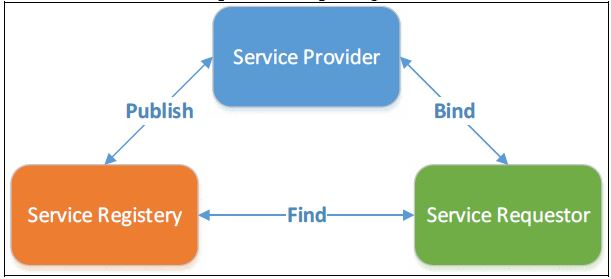
\includegraphics[width=1\textwidth]{figures/arsitektur.JPG}}
\caption{Arsitektur web service.}
\end{figure}
terdapat tiga komponen utama dari web service, komponen komponen tersebut antara lain :
service Provider, Service Requestor, Service Registry 
service Provider adalah penyedia web service yang berfungsi menyediakan kumpulan webService yang dapat diakses oleh USER atau pengguna.
Service Requestor Adalah aplikasi yang bertindak sebagai pengguan yang melakukan permintaan layanan berupa WebService kepada Service Provider.
Service Registry Adalahtempat dimana service provider mempublikasikan layanannya. pada arsitektur Webservice, service registry bersipat opsional.\cite{kurniawan2015implementasi}


ini merupakan contoh tabel \ref{table:contoh} ukuran kecil.
\begin{table}[h]
\caption{Bahasa pemerograman yang sering digunakan di Frontend}
\centering
\begin{tabular}{ccccc}
\hline
one&two&three&four&five\\
\hline
Java&Phyton&PHP&Javascript&C++\\
\hline
\end{tabular}
\label{table:contoh}
\end{table}





\chapter[Pengertian Web Service]
{pengertianwebservice}
%Resume tentang Pengertian Web Service

%Kelompok 2 D4 TI / 2B

%Alwan Suryansah				1164033 
%Dinda Ayu Pratiwi				1164034
%Kurnia Sandi					1164042
%Teduh Sanubari					1164054
%Wildan Khaustara Wijaksana		1164058


\section{Definisi}

\subsection{Hartati Deviana}

	Web service adalah suatu komponen perangkat lunak self-containing dan aplikasi modular self-describing yang dapat disiarkan, dialokasikan, dan dijalankan di dalam web. Web service adalah teknologi yang mentransformasikan kemampuan internet dengan cara menambahkan beberapa kemampuan seperti kemampuan transactional web. Apa itu Transactional Web? Transactional Web yaitu kemampuan web dalam hal saling berinteraksi dengan pola program-to-program (P2P). Fokus web selama ini didominasi oleh komunikasi program-to-user dengan interaksi business-to-consumer (B2C), sedangkan transactional web akan didominasi oleh P2P dengan interaksi business-to-business (B2B). \cite{deviana2013penerapan}.

	Web service adalah suatu sistem perangkat lunak yang dirancang untuk mendukung interoperabilitas dan interaksi antar sistem pada suatu jaringan. Web service digunakan sebagai suatu fasilitas yang disediakan oleh suatu web site untuk menyediakan layanan (dalam bentuk informasi) kepada sistem lain, sehingga sistem lain dapat berinteraksi dengan sistem tersebut melalui layanan-layanan (service) yang disediakan oleh suatu sistem yang menyediakan web service. Web service menyimpan data informasi dalam format XML, sehingga data ini dapat diakses oleh sistem lain walaupun berbeda platform, sistem operasi, maupun bahasa compiler. 

\subsection{Richards Robert}

	Web service merupakan salah satu implementasi dari teknologi XML (Extensible Markup Language) pada proses pertukaran antara (data exchange) platform yang berbeda sercara berbeda.

\textit{"A Web service is a software system designed to support interoperable machine-to-machine interaction over a network. It has an interface described in a machine-processable format(specifically WSDL).Other systems interact with the Web service in a manner prescribed by its description using SOAP messages, typically conveyed using HTTP with an XML seriali zation in conjunction with other Web-related standards"}.

Menurut Richards, web service dapat digunakan untuk berkomunikasi antara mesin satu dengan mesin yang lain melalui interface perantara yang umumnya berupa WSDL(Web Service Definition Language), layanan ini biasa bekerja pada protokol HTTP dengan bentuk response dan request berupa SOAP messange. SOAP (Simple Object Access Protocol) adalah standar untuk bertukar pesan-pesan berbasis XML melalui jaringan komputer atau sebuah jalan untuk program yang berjalan pada suatu sistem operasi (OS) untuk berkomunikasi dengan program pada OS yang sama maupun berbeda dengan menggunakan HTTP dan XML sebagai mekanisme untuk pertukaran data. Format SOAP message adalah mengikuti frame XML yang terstandarisasi \cite{ihya2011pembuatan}. 

\subsection{Chen, Xi dan Zheng, Zibin dan Yu, Qi dan Lyu, Michael R}

	Web Service adalah komponen perangkat lunak yang terintegrasi untuk mendukung interaksi antar mesin dengan mesin yang lainya ( komputer ) antar jaringan , layanan web service telah banyak digunakan untuk membangun suatu aplikasi yang berorientasi dengan layanan industri dan akademisi dalam beberapa tahun trakhir , jumlah layanan web yang tersedia untuk umum terus meningkat di internet , Namun  ini menyulitkan pengguna untuk memilih layanan yang tepat di antara banyaknya layanan web services\cite{chen2014web}.

\subsection{Witono, Timotius and Susanto, Raphael}

	Pengertian sederhana web service adalah aplikasi yang dibuat agar dapat dipanggil atau diakses oleh aplikasi lain melalui internet atau intranet dengan menggunakan XML sebagai format pengiriman pesan. Web service digunakan saat pengguna akan mentransformasi sebuah logik atau sebuah class dan objek yang terpisah dalam satu ruang lingkup yang menjadi satu, sehingga tingkat keamanan dapat ditangani dengan baik\cite{witono201511}.

\subsection{Kurniawan, Erick}

	Web Service adalah layanan yang tersedia di Internet. Web Service menggunakan format standar XML untuk pengiriman pesannya. Web Services juga tidak terikat kepada bahasa pemrograman atau sistem operasi tertentu (Ethan Cerami, 2002). Web Services adalah antar muka yang mendeskripsikan koleksi yang dapat diakses dalam jaringan menggunakan format standar XML untuk pertukaran pesan. Web Services mengerjakan tugas yang spesifik. Web Services dideskripsikan menggunakan format standar notasi XML yang disebut services description (Gottschalk, 2002)\cite{chen2014web}.

\subsection{Sarbini, Riska Nurtantyo}

	Web service merupakan satuan diskrit dari fungsionalitas programatis yang diekspos 
kepada client via protokol komunikasi, dan format data standar bernama HTTP dan 
XML. Protokol ini mengatasi masalah komunikasi lintas internet dan lintas 
firewall tanpa beralih ke solusi superior yang memerlukan port-port komunikasi 
tambahan yang harus dibuka untuk akses eksternal. Dikarenakan web service mamiliki fungsi untuk menformat dan menguraikan pesan XML\cite{sarbini2015pengembangan}. 

\subsection{M. Shalahuddin dan Rosa A.S.}

	Web Service merupakan suatu sistem yang menyediakan pelayanan yang dibutuhkan oleh klien. Klien dari web service tidak hanya berupa aplikasi web, tetapi juga bisa sebuah aplikasi enterprise. Jadi web service tidak sama dengan web server, bahkan sebuah aplikasi web pada web server dapat menjadi klien dari web service\cite{inayah2014aplikasi}.

\subsection{Gottschalk (2002)}

	Web Service adalah teknologi yang mengubah kemampuan internet dengan menambahkan kemampuan transactional web, yaitu kemampuan web untuk saling komunikasi dengan pola program to program (P2P). Fokus web selama ini didominasi oleh komunikasi program to user dengan interaksi business to costumer (B2C), sedangkan stransactional web akan didominasi oleh P2P dengan interaksi business to business\cite{fauziah2014aplikasi}.


\subsection{Slameto, Andika Agus}

	Web service adalah suatu sistem perangkat lunak yang dirancang untuk mendukung interoperabilitas dan interaksi antar sistem pada suatu jaringan. Web service digunakan sebagai suatu fasilitas yang disediakan oleh suatu web site untuk menyediakan layanan (dalam bentuk informasi) kepada sistem lain, sehingga sistem lain dapat berinteraksi dengan sistem tersebut melalui layanan-layanan (service)yang disediakan oleh suatu sistem yang menyediakan web service. Web service menyimpan data informasi dalam format XML, sehingga data ini dapat diakses oleh sistem lain walaupun berbeda platform, sistem operasi, maupun bahasa compiler\cite{slameto2015penerapan}.

\subsection{Jurnal Masyarakat Informatika}

	Web service adalah antarmuka yang mendeskripsikan sekumpulan operasi yang dapat diakses dalam sebuah jaringan melalui pesan XML yang telah distandartkan.xml iyalah bahasa markup yang sudah terintregrasi dengan web service. W3C mendefinisikan web service sebagai sebuah sistem perangkat lunak yang dirancang untuk mendukung inter operasi mesin ke mesin di sebuah jaringan.  Web service merupakan komponen perangkat lunak loosely coupled, dapat diguna ulang, membungkus fungsionalitas diskret, didistribusikan, dan diakses secara programatik melalui protokol internet standart . dan sangat di di perhatikan di bidang informatika \cite{saputra2integrasi}.

\subsection{Jurnal Sistem dan Teknologi Informasi}

	Web service menurut World Wide Web Consortium (W3C) (2004), organisasi yang mengembangkan standar-standar dalam dunia web, mendefinisikan web service sebagai "\textit{“a software system designed to support interoperable machine-to-machine interaction over a network. It has an interface described in a machine-processable format (specifically WSDL). Other systems interact with the Web service in a manner prescribed by its description using SOAP messages, typically conveyed using HTTP with an XML serialization in conjunction with other Web-related standards.” }"(Lucky,2008).

Berdasarkan definisi dari W3C dapat disimpulkan bahwa web service merupakan aplikasi yang dibuat agar dapat dipanggil atau diakses oleh aplikasi lain melalui internet maupun intranet dengan menggunakan XML sebagai format pengiriman pesan\cite{prasetya2013perancangan}.

\subsection{Pengertian Web Service menurut Hartono, Fajar Fani and Hendry, H and Somya, Ramos}

	Web Service dapat diartikan sebuah antar muka atau dalam bahas inggris yaitu interface  yang berarti menggambarkan sebuah sekumpulan operasi-operasi yang kemudian dapat diakses melalui jaringan, misalnya internet dalam bentuk pesan “Extensible Markup Language (XML)”. Web Service juga menyediakan standar komunikasi dalam berbagai software yang berbeda-beda, dan dapat berjalan di berbagai platform maupun framework\cite{hartono2013aplikasi}.

\subsection{Pengertian Web Service Menurut Kasaedja, Bramwell A and Sengkey, Rizal and Lantang, Oktavian A}

	O’Reilly menerbitkan sebuah buku, David A Chappel dan Tyler Jewell sebagai penulis mengartikan bahwa web service adalah suatu kumpulan logika bisnis dalam internet yang dapat di akses melalui protocol internet. Dalam buku tersebut juga dijelaskan bahwa terdapat tiga komponen teknologi dalam Web service yaitu, Simple Object Acces Protocol (SOAP), Web Service Description Language (WSDL), dan Universal Description, Discoveri, Integration (UDDI)\cite{kasaedja2014rancang}.

\subsection{Hamdani, Hamdani and Haviluddin, Haviluddin and Darmawangsa, Ngurah Satria}

	Web service diartikan sebagai sebuah antar muka (interface) yang menggambarkan sekumpulan operasi-operasi yang dapat diakses melalui jaringan, misalnya internet, dalam bentuk pesan XML. Web service diartikan sebagai sepotong atau sebagian informasi atau proses yang dapat diakses oleh siapa saja, kapan saja dengan menggunakan piranti apa saja, tidak terikat dengan sistem operasi atau bahasa pemrograman yang digunakan.

\subsection{Novi Nuari}

	Webservice ialah suatu sistem perangkat lunak yang dibangun guna mendukung interaksi antar mesin dalam suatu jaringan. Webservice digunakan sebagai suatu fasilitas yang disediakan oleh suatu website untuk menyediakan layanan (dalam bentuk informasi) kepada mesin lain, sehingga mesin lain dapat berinteraksi dengan mesin tersebut melalui layanan-layanan (service) yang disediakan oleh provider\cite{nuari2014perancangan}.

\subsection{Wellem, Theophilus}

	Web service merupakan suatu software sistem yang mendukung interaksi yang interoperable dari machine to machine melalui jaringan (World World Wide Consortium).  (Stencil Group). Dengan suksesnya Web service sebagai suatu standar teknologi software, memberikan peluang yang besar untuk pengembangan aplikasi terdistribusi melalui Internet.
Web service sebagai suatu standar teknologi software, memberikan peluang yang besar untuk pengembangan aplikasi terdistribusi melalui Internet. Saat ini Web service tidak hanya dapat diakses melalui komputer saja, tetapi juga dapat diakses melalui mobile device, seperti telepon seluler dan PDA, sehingga memungkinkan diciptakannya layanan mobile menggunakan Web service dan aplikasi mobile yang menggunakan Web service ini\cite{wellem2015perancangan}.

\subsection{Jurnal Informatika Kenali, Eko Win }

	Menurut Gerami (2002) web services adalah suatu layanan-layanan yang disediakan oleh internet, dengan menggunakan pengiriman pesan format Extensible Markup Language (XML), dan tidak saling bergantung pada satu sistem operasi atau Bahasa pemrograman. Komponen dalam web service memiliki 3 arsitektur, dan masing-masing komponen tersebut adalah Service provider, Service requestor, dan Service registry\cite{kenali2015desain}. 

\subsection{Sigit, Haris Triono and Sulistiyono, Sulistiyono}

	Web Service adalah bagian dari perangkat lunak yang membuat dirinya tersedia melalui internet dan menggunakan sistem pesan XML standar. XML digunakan untuk mengkodekan semua komunikasi ke Web Service. Misalnya, klien memanggil Web Service dengan mengirim pesan XML, kemudian menunggu tanggapan XML yang sesuai. Karena semua komunikasi ada dalam XML, Web Service tidak terkait dengan sistem operasi atau bahasa pemrograman manapun. Web Service adalah kumpulan protokol dan standar terbuka yang digunakan untuk pertukaran data antara aplikasi atau sistem\cite{sigit2017desain}.  

\section{Manfaat}

Layanan web memungkinkan penyedia layanan dan vendor untuk menjual layanan mereka dengan memublikasikannya
Yang di akses melalui World Wide Web.
Manfaat dari layanan web kita dapat berbagi data walaupun memiliki jarak yang jauh dan dapat mempermudah membagi suatu data dalam sebuah pekerjaan
interoperabilitas. Manfaat ini berasal dari antarmuka XML standar dan deskripsi akses
diberikan oleh WSDL (Web Services Description Language). Deskripsi WSDL sangat membantu dalam perusahaan
integrasi aplikasi, integrasi B2B (menyelesaikan tantangan antara bisnis dan bisnis partner, seperti customer, supplier, bank, dan jasa transportasi ) \cite{ferris2003web}.

\section{Arsitektur Web service}

\subsection{\textit{Service Oriented Architecure (SOA)} }

	Konsep arsitektur yang mendasari teknologi Web service adalah Service Oriented Architecure (SOA), SOA mendefinisikan 3 peran berbeda yang menunjukkan peran dari masing-masing komponen dalam system, yaitu (W3C, 2004) :
\begin{itemize}
\item \textit{Service provider}, yaitu suatu entitas yang menyediakan interface terhadap sistem yang menjalankan suatu sekumpulan tugas tertentu.
\item \textit{Service requestor}, yaitu suatu entitas yang meminta/memperoleh (dan menemukan) \textit{software service} dalam rangka meyelesai kan suatu tugas tertentu atau menyediakan solusi bisnis tertentu.
\item \textit{Service registry}, yaitu entitas yang bertindak sebagai penyimpan (\textit{repository}) suatu \textit{software service} yang dipublikasikan oleh \textit{service provider}\cite{hidayat2014penerapan}.
\end{itemize}

\subsection{Jurnal Masyarakat Informatika}

	Web service dibangun dari tiga komponen unsur utama, yaitu service provider, service registry, dan service requestor. Komponen-komponen tersebut saling berinteraksi melalui komponen web service itu sendiri, yang berupa deskripsi dan implementasi layanan dan prasarana. Dan juga terdapat tiga macam operasi yang memungkinkan komponen komponen tersebut untuk dapat saling berinteraksi, yaitu publish, find, dan bind. Keterkaitan antara peran, operasi, dan komponen web service \cite{saputra2integrasi}.

\subsection{Arsitektur RESTful Web services}

	Berikut merupakan langkah-langkah yang dilakukan dalam model dasar RESTful Web services (HostBridge, 2009):
\begin{enumerate}
\item Query Request Provider melalui HTTP dengan menggunakan URI (Uniform Resource Identifier). Request menggunakan methods (metode) HTTP untuk menentukan apakah request tersebut dimaksudkan untuk Create (menciptakan), Read (membaca), Update (memperbarui), atau Delete (menghapus) data.
\item HostBridge mengembalikan sebuah dokumen dalam bentuk XML untuk Requester (pemohon) dengan CICS data enclosed\cite{arsana2014rancang}.
\end{enumerate}



\section{Kesimpulan}

	Dari berbagai definisi tersebut dapat disimpulkan bahwa web service merupakan middleware sebuah internet yang memungkinkan berbagai sistem untuk saling berkomunikasi tanpa terpengaruh pada platform. Web service membungkus operasi-operasi ke dalam sebuah antarmuka yang ditulis dalam notasi XML. Antarmuka ini menyembunyikan detil implementasi dari layanan. Pertukaran informasi yang terjadi dalam web service juga menggunakan pesan dalam format XML \cite{saputra2integrasi}.




\chapter[Port]
{Port}
\input{section/1port.tex}


\chapter[Aplikasi Web Service]
{Aplikasi Web Service}
\input{section/1aplikasiwebservice.tex}

\chapter[Protokol]
{Protokol}
%Resume Protokol Kelompok 3 D4TI2B
%\begin{enumerate}
%\Fikri aldi nugraha                  1164038
%\Nur Arkhamia Batubara               1164049 
%\Miftahul Hasanah                    1164046 
%\Si Made Angga Dwitya P              1164053 
%\Widary Anggraini Mindo V Siahaan    1164057
%\end{enumerate}

\section{Pengenalan Protokol} 

Dalam jaringan computer, protocol merupakan konvensi yang disepakati untuk komunikasi antarkomputer. Selanjutnya, protocol TCP/IP 
mendefinisikan bagaimana pesan dikirimkan melalui internet, sedangkan protocol FTP, yang dibangun menggunakan protocol TCP/IP,mendefinisikan pesan-pesan FTP dikirim dan diterima. Dan dalam sistem jaringan dan komunikasi, ada spesifikasi prosedur yang diikuti saat akan mengirim atau menerima data. Protocol menentukan format, waktu, urutan, dan system pengecekan kesalahan yang digunakan.

Apabila dua buah system yang saling berkomunikasi, hal pertama yang dibutuhkan adalah kesamaan bahasa yang digunakan. Sehingga dapat 
memahami alur proses komunikasi. Lain halnya apabila dua buah system saling berkomunukasi dengan bahasa yang berlainan, tentunya dua 
system tersebut tidak akan saling memahami. Untuk itu, system tersebut membutuhkan sebuah mekanisme pengaturan bahasa yang dapat 
dipahami oleh dua buah system tersebut sehingga pertukaran informasi antar system akan dapat terjadi dengan benar. Aturan bahasa 
komunikasi ini sering disebut protocol komunikasi. 
 
Suatu standar pertukaran informasi. Komputer dengan system operasi dan software berbeda dapat saling berkomunikasi melalui internet 
karena pengadopsian protokol. Seperangkat aturan umum (atau bahasa) yang mengijinkan komputer-komputer untuk saling berkomunikasi. 
Protokol yang standart adalah TCP/IP (Transmission Control Protocol/Internet Protocol). Web menggunakan server protokol HTTP agar 
komputer dapat mengakses file , melakukan pencetakan, berkomunikasi, dan menyediakan layanan lain bagi user lain dalam jaringan.    
 Seperangkat aturan formal yang mendeskripsikan bagaimana cara mentransfer data, terutama dalam jaringan. Protocol level bawah
 mengobservasi standar elektrikal dan fisikal, perintah bit dan byte, pendeteksian transmisi dan kesalahan, serta koreksi terhadap 
 aliran bit. Protocol level atas berkaitan dengan pemformatan data, meliputi sintax pesan, terminal dari dialog computer, susunan 
 karakter, urutan pesan, dan lain-lain.
 
 Ketika data ditransmisikan diantara dua atau lebih peralatan, diperlukan sesuatu yang dapat menjaga control agar data tetap utuh, yaitu 
 suatu deskripsi formal mengenai pesan dan aturan yang harus diikuti oleh dua computer yang ingin bertukar pesan. Protocol dapat 
 mendeskripsikan detal dari interface mesin ke mesin level bawah (cara bagaimana dua program mentransfer file melalui internet).
 
 \section{Elemen Penting Protokol}
 \begin{enumerate}
 \item  Syntax, mengacu pada struktur atau format data, yang mana dalam urutan tampilannya memiliki makna tersendiri.
 \item  Semantics, mengacu pada maksud setiap section bit. Dengan kata lain adalah bagaimana bit-bit tersebut terpola untuk dapat 
 diterjemahkan.
 \item  Timing, mengacu pada 2 karakteristik, yakni kapan data harus dikirm dan seberapa cepat data tersebut dikirim.
 \end{enumerate}

 
 \section{Pengertian Protokol}
Protokol merupakan aturan dalam melakukan pengiriman data (berupa blok-blok data) dari sebuah node jaringan ke node jaringan lain.
Protokol merupakan sarana komunikasi antara mesin melalui jaringan yang terstandarisasi. Protokol mengizinkan data untuk ambil bagian 
dalam transmisi kilat, kemudian ditransmisikan, lalu dikumpulkan kembali sesuai arah dengan perintah yang benar. 
Protokol digunakan untuk mendeteksi kesalahan, tipe kompresi, dan bagaimana receiver (penerima) mengindikasikan bahwa pesan telah 
diterima. 
Protokol dapat mendeskripsikan detail level bawah dari interface machine to machine atau pertukaran level atas antara program alokasi. 
Protokol level bawah meliputi observasi terhadap standar elektrik dan fisik, perintah bit dan byte, pendeteksian transmisi dan 
kesalahan, dan koreksi aliran bit. 
Protokol level atas berkaitan dengan pemformatan data, meliputi sintaks pesan, dialog dari terminal ke komputer, dan pengurutan pesan. 

Protocol merupakan seperangkat aturan komunikasi dimana dalam sebuah hubungan telekomunikasi dapat digunakan untuk menerima sinyal. 
Dalam  koneksi telekomunikasi tersebut protocol dapat  koita bagi menjadi 7 level. Salah satunya yaitu hardware protocol telepon dan 
berupa end point dalam sebuah program komunikasi dalam computer yang sama atau memiliki lokasi yang berbeda-beda. Jadi kedua end point 
tersebut harus dapat mengenali satu sama lain dan mengobservasi protocol.

 \section{Jenis-Jenis Protokol}
Protokol jaringan adalah berbagai protokol yang terdapat dari lapisan  teratas sampai terbawah yang ada dalam sederetan protocol.
Di pandang dari sudut komunikasi data,ada beberapa protokol yang banyak digunakan pada jaringan computer, di antaranya:

 \subsection{TCP/IP}
TCP/IP merupakan protokol standar pada jaringan internet yang tidak tergantung pada jenis computer yang digunakan.
Barangkali perlu dicatat bahwa TCP/IP adalah perlengkapan standar pada sistem operasi Unix dan turunannya.
Saat ini mesin novell,SUN maupun Machintosh sudah dilengkapi protokol standar TCP/IP ini.

Protocol adalah spesifikasi forma yang mendefenisikan prosedur-prosedur yang harus diikuti ketika mengirim dan menerima data (Wermer, 
1996). Protocol mendefenisikan jenis, waktu, urutan dan pengecekan kesalahan yang digunakan dalam jaringan. Transmission control 
protocol/internet protocol (TCP/IP) merupakan protocol untuk mengirim data antar computer pada jaringan. Protocol ini merupakan protocol 
yang digunakan untuk akses internet dan digunakan untuk komunikasi lobal. TCP/IP terdiri atas dua protocol yang terpisah. TCP/IP 
menggunakan pendekatan lapisan (layer) pada saat membangun protocol ini. Dengan adanya pendekatan berlapis ini memungkinkan dibangunnya 
beberaa layanan kecil untuk tugas-tugas khusus.

TCP/IP terdiri dari lima layer, yaitu :
\begin{enumerate}
\item   Layer Application, di dalam layer ini aplikasi seperti FTP, Telnet, SMTP, dan NFS dilaksanakan.
\item   Layer Transport, di dalam layer ini TCP dan UDP menambah data transport ke paket dan melewatkannya ke layer Internet.
\item    Layer Internet, Layer ini mengambil paket dari layer transport dan menambahkah informasi alamat sebelum mengirimkankannya ke layer network interface.
\item     Layer Network Interface, di dalam layer ini data dikirim ke layer physical melalui device jaringan.
\item     Layer Physical, layer ini merupakan system kabel yang digunakan untuk proses mengirim dan menerima data.
\end{enumerate}

\begin{table} [h]
\begin {tabular} {|cc|}
\hline
Lapisan Model OSI & \\
\hline
Application atau Presentation & \\
\hline
Session & \\
\hline
Transport & \\
\hline
Network & \\
\hline
Data Link atau Physical & \\
\hline
\end{tabular}
\end{table} 
  
 \subsection{UDP(User Datagram Protocol)}
UDP adalah salah satu protokol dari layer transport yang merupakan layer ketiga dalam model TCP/IP Layer.
UDP mengirim paket berupa datagram yang terdiri dari sebuah header kecil dan data pengguna UDP memiliki karakteristik connectionless, 
yaitu pengirim mengirimkan paket secara langsung tanpa membangun koneksi ke server. 
Keunggulan lain dari UDP yaitu fleksibel karena rute pengiriman paket dapat dengan mudah diubah, apabila terjadi antrian pada suatu rute tertentu 
 
 \subsection{SNMP(Simple Network Management Protocol)}
SNMP adalah sebuah protokol aplikasi pada jaringan TCP/IP yang menangani manajemen jaringan. 
Protokol ini didesain sehingga pengguna dapat dengan mudah memantau kondisi jaringan komputer. 
Pemantauan kondisi jaringan dapat dilakukan dengan cara pengumpulan nilai-nilai informasi dari kondisi jaringan secara jarak jauh atau 
menggunakan satu pusat pengamatan.
  
 \subsection{AppleTalk} 
Protokol AppleTalk dibuat oleh sebuah perusahann Apple Computer, digunakan pada jaringan dengan komputer mesin Apple, dipublikasikan 
pada tahun 1985. Teknologi Protokol ini milik Apple. Metode akses LocalTalk berfungsi sebaik Ethernet dan Token Ring. 2 metode yaitu 
Manajemen jaringan AppleTalk dan metode akses LocalTalk telah disatukan ke dalam semua mesin Macintosh dan LaserWriter. Bersama produk 
lainnya dari Apple dan mesin tipe lain, AppleTalk dapat kita aplikasikan  baik di PC, VAX maupun  pada workstation UNIX. Sejak AppleTalk 
diperkenalkan (setelah model OSI), protocol Appletalk merupakan routable protocol yang terkandung dalam sebuah network layer (OSI layer 
3). 

\subsection{IPX/SPX(Internet Packet Exchgange/Sequenced Packet)}  
IPX dan SPX adalah protocol standar pada jaringan Novell Netware,untuk mengatasi masalah internetworking pada jaringan 
PC.Kenyataanya,sering kali IPX dijalankan berkaitan dengan TCP/IP karena menguntungkan.Novell Netware merupakan sistem operasi jaringan 
komputeryang dirancang untuk mengaitkan PC ke dalam jaringan antar-PC,yangdapat membuat resource harrdisk dari server dapat digunakan 
bersama.Hubungan antar-client menjadi transparan(antara yang satu dengan lainnya).

Pada tahun 1980-an hingga permulaan tahun 1990-an,sistem operasi ini menguasai hamper seluruh pasaran jaringan computer.
Paket Internetnetwork Packet Exchange(IPX) alamat jaringan dan dapat melakukan pengaturan(route dari satu jaringan ke jaringan 
lain.Sebuah paket IPX terkadang dapat terlewatkan ketika terjadi crossing network, sehingga IPX tidak menjamin pengiriman pesan akan 
terselesaikan. Salah satu dari aplikasi yang tersedia adalah control yang berarti prttokol SPX NetWare harus digunakan. Protokol IPX ini 
berjalan pada layer 3 dan 4 dari model OSI.

AppleTalk Filling Protocol (AFP) adalah sebuah protocol yang digunakan untuk mengatur penerimaan file dan pengiriman file dari komputer 
Apple.
Zone Information Protocol (ZIP) merupakan sebuah  protocol yang digunakan  untuk mengatur sebuah  daerah (zone) yang dibuat  oleh 
jaringan AppleTalk. Zip berfungsi untuk memetakan nomor network ke suatu zone.
Routing Table Maintenance Protokol (RTMP) adalah sebuah  protocol yang digunakan untuk  routing bagi AppleTalk yang berjenis distance 
vector.
Name Binding Protokol (NBP) dapat kita gunakan untuk mengadakan translasi suatu nama dari alamat AppleTalk seperti DNS di TCP/IP).

\subsection{Voice Over Internet Protocol(VoIP)}
Voice Over Internet Protocol merupakan suatu teknologi yang dapat mengirimkan paket suara melalui jaringan Internet Protocol . Jaringan 
Internet Protocol (IP) ini  sendiri merupakan jaringan komunikasi data yang berbasis packet-switch, sehingga dalam berkomunikasi 
menggunakan protocol VoIP berarti menggunakan jaringan internet untuk melakukan komunikasi. Protocol ini juga sering disebut Ip 
Telephony, Internet Tellephony atau Digital Phone.

Pada teknologi VoIP memerlukan protocol agar bisa saling berhubungan dan berkomunikasi, beberapa protocol yang dapat digunakan dalam 
membangun suatu jaringan VoIP adalah protocol H.323 dan Session initiation Protocol (SIP). Pada dasarnya kedua protocol tersebut 
mempunyai peranan yang sangat penting dalam membangun komunikasi menggunakan VoIP. Kualitas suara pada VoIP sangat dipengaruhi oleh 
beberapa parameter, diantaranya adalah bandwidth, delay, filter dan packet loss.

Konsep cara kerja VoIP yaitu dengan melakukan pengiriman sebuah sinyal secara digital, sebelum proses transmisi (pengiriman) dilakukan 
data yang berupa sinyal analog akan dikonversikan terlebih dahulu dengan ADC (Analog to Digital Converter) menjadi bentuk data digital. 
Setelah proses konversi dilakukan data digital akan ditransmisikan ke sumber tujuan.Setelah sampai, data sinyal digital tersebut akan 
dikonversi kembali menjadi data sinyal analog dengan DAC (Digital to Analog Converter) sehingga dapat diterima oleh sumber tujuan 
sesuai dengan data sinyal yang ditransmisikan.

Ada empat komponen pada VoIP yang pertama user agent, merupakan suatu komponen yang digunakan olah pengguna untuk memulai dan menerima 
suatu sesi komunikasi Dalam VoIP. Yang kedua Proxy, merupakan aplikasi server yang mengatur jaringan VoIP. Kemudian protocol, protocol 
merupakan aturan komunikasi yang terjadi Antara user agent dengan proxy. Yang terakhir Codec, codec teknologi yang mempaketkan data 
voice kedalam format lain sehingga menjadi lebih teratur dan mudah dipaketkan.

\subsection{NetBIOS}
NetBIOS digunakan dalam Microsoft Work Group dengan metode peer to peer. Protockol NetBIOS memberikan layanan pada session layer dan 
transport layer (layer 4 dan 5 model OSI). NetBIOS tidak menyediakan format frame untuk kelebihan transmisi jaringan dikarenakan adanya 
berbagai macam perbedaan implementasi NetBIOS yang terjadi. Sebagai contoh, Artisoft LANtastic menggunakan sebuah versi dari NetBIOS 
untuk transmisi antara client dan server. Format frame disusun di NetBEUI, yang digunakan pada semua system operasi Windows yang 
mendukung jaringan.

\subsection{SNA (Systems Network Architecture)}
SNA diperkenalkan pada tahun 1974. Dulunya adalah arsitektur yang terpusat dengan sebuah host komputer dan mengatur banyak terminal. 
SNA mengalami banyak pengembangan,seperti APPN dan APPX(LU 6.2), yang telah mengadaptasi SNA ke dalam komunikasi peer to peer dalam 
lingkungan komputer terdistribusi. SNA Layers diterapkan dilapisan paling bawah yang mengirim paket dari satu stasiun ke stasiun yang 
lain. Lapisan ini merupakan kumpulan beberapa protocol. Walaupun SNA banyak mempengaruhi model OSI, namun ada beberapa perbedaan dalam 
implementasinya.

\subsection{ICMP(Internet Control Message Protocol)}
ICMP merupakan protokol yang digunakan untuk melakukan tes koneksi dari sebuah host ke host yang lain.
ICMP melakukan tes koneksi dengan mengirimkan sebuah request packet ke host tujuan dengan menggunakan IP address.
ICMP merupakan protocol pesan pada TCP/IP. ICMP menyediakan pesan control dan error yang digunakan oleh ping dan traceroute yang bekerja pada layer jaringan.

\subsection{SNMP(Simple Network Management Protocol)}
SNMP adalah sebuah protocol yang kita pakai untuk  dapat memantau dan mengontrol jaringan dari tempat lain(jauh). Data dilewatkan dari 
SNMP agent yaitu hardware atau software yang melaporkan suatu aktivitas/proses kepada beberapa perangkat jaringan lainnya seperti hub, 
router, maupun bridge, .Monitoring ini dapat kita  dilakukan melalui console dari workstation. Agent mengembalikan informasi yang 
terdapat pada MIB (management information Base) dimana merupakan sebuah struktur data yang menggambarkan data apa saja yang kita 
dapatkan  dari perangkat dan apa  saja yang dapat dikontrol(dimatikan,dihidupkan,dall).

\subsection{SLIP (Serial Line IP)}
Dalam sebuah data link protocol untuk akses ke jaringan TCP/IP. Biasanya digunakan untuk mendapatkan akses internet.SLIP mengirimkan 
paket IP melalui serial link (dial up atau private line). AX.25 adalah turunan dari protocol x.25 akan tetapi digunakan sebagai protocol 
penghubung dalam jaringan paket radio. Selain itu sebetulnya masih ada kelurga protocol yang lain, seperti yang dikembangkan oleh 
OSI/ISO: X.25/X.75/X.400 yang juga mulia digunakan oleh beberapa institusi.

UUCP (Unix-to-Unix Copy Program), pada mulanya untuk mengirimkan file antarmesin Unix. File-file itu dapat berupa surat elektronik (e-
mail) maupun konferensi elektronik (news). Solusi ini baik untuk pengembangan jangka panjang sebuah jaringan computer, akan tetapi dapat 
digunakan untuk solusi sementara yang bersifat darurat. Sayang segala informasi tentang protocol ini harus dibeli keke ISO. Hal ini 
dapat berkembang ISO/OSI tersendat, tidak seperti TCP/IP.

\subsection{FTP (File Transfer Protocol)}
FTP adalah sebuah protokol Internet yang berjalan di dalam lapisan aplikasi yang merupakan standar untuk pentransferan berkas antar 
mesin-mesin dalam sebuah Internetwork. 
FTP didefinisikan sebagai sebuah protokol untuk mengirim dan menerima file antara host (dalam Advanced Research Project Agency Network 
(ARPANET). 
Fungsi utama dari FTP adalah mengirim dan menerima file dengan efisien dan handal antara host dan mengijinkan penggunaan yang nyaman 
dari kemampuan untuk penyimpanan file secara remote.

\subsection{Elemen yang terdapat pada protokol}
Elemen penting protocol adalah syntax,semantics,dan timing.
-Yang pertama Syntax maksudnya yaitu dipusatkan pada struktur atau format data, yang mana dalam urutan tampilannya memiliki makna 
tersendiri. Sebagai contoh sebuah protocol sederhana akan memilki urutan pada 8 bit pertama sebagai alamat pengirim,dan bit selanjutnya 
itu adalah informasi tersendiri. 
-Yang kedua yaitu semantic yang mengacu pada maksud setiap section pada bit dapat dikatakan bahwa beberapa bit bit tersebut terpola  
sehingga bit bit tersebut dapat  kita diterjemahkan.
-Yang ketiga yaitu timing, timing lebih dipusatkan kepada 2 karakteristik,yaitu  kapan suatu data tersebut seharusnya dikirimkan dan 
yang kedua seberapa cepat data tersebut dapat kita kirim.



% contoh aplikasi web service
% web service
% protokol
% port

% HTTP
% URL
% POST
% GET



\bibliographystyle{IEEEtran}.
\bibliography{references}.

\printindex

\end{document}
